\documentclass[12pt, a4paper]{article}
\usepackage[utf8]{inputenc}
\usepackage{hyperref}
\usepackage{graphicx}
\usepackage{listings}
\usepackage{xcolor}

\definecolor{codegreen}{rgb}{0,0.6,0}
\definecolor{codegray}{rgb}{0.5,0.5,0.5}
\definecolor{codepurple}{rgb}{0.58,0,0.82}
\definecolor{backcolour}{rgb}{0.95,0.95,0.92}

\lstdefinestyle{mystyle}{
    backgroundcolor=\color{backcolour},   
    commentstyle=\color{codegreen},
    keywordstyle=\color{magenta},
    numberstyle=\tiny\color{codegray},
    stringstyle=\color{codepurple},
    basicstyle=\ttfamily\footnotesize,
    breakatwhitespace=false,         
    breaklines=true,                 
    captionpos=b,                    
    keepspaces=true,                 
    numbers=left,                    
    numbersep=5pt,                  
    showspaces=false,                
    showstringspaces=false,
    showtabs=false,                  
    tabsize=2
}

\lstset{style=mystyle}

\hypersetup{
    colorlinks=true,
    linkcolor=black,
    urlcolor=cyan,
}

\graphicspath{{img/}}


\title{\textbf{Elaborato di Intelligenza Artificiale} \\ Implementazione di una Simulazione con Modelli di Reti Neurali Utilizzando l'Ambiente di Sviluppo Python}
\author{Soldà Matteo --- 1226319}
\date{\today}

\begin{document}

\begin{figure}
    \centering
    \includegraphics[width=0.50\textwidth]{Logo_Università_Padova}
\end{figure}

\maketitle

\newpage
\begin{abstract}
Nel presente elaborato verrà implementata una simulazione tramite modelli di reti neurali utilizzando l'ambiente di sviluppo Python.\\
La simulazione si baserà sul database \textit{MNIST}, riguardante il riconoscimento di numeri manoscritti, fornitoci durante la terza esercitazione pratica.\\
L'obiettivo di tale documento è di rispondere a tre domande essenziali: definire le cifre più difficili da riconoscere, quantificare la variazione di accuratezza dovuta all'inserimento di rumore nel \textit{training pattern} e la variazione dell'accuratezza di riconoscimento sul \textit{testing pattern} riducendo drasticamente le dimensioni del \textit{training pattern}.    
\end{abstract}

\newpage
\tableofcontents

\newpage
\section{Introduzione}
In questo elaborato si prenderà in considerazione uno dei problemi più famosi che vengono sottoposti alle intelligenze artificiali: il riconoscimento di numeri manoscritti.
La simulazione chè verrà presentata si baserà sul dataset \textit{MNIST}, il quale contiene 70.000 immagini, con relative etichette, di cifre comprese tra 0 e 9 scritte a mano.\\
Per risolvere il problema sopra descritto, utilizzeremo una variante convoluzionale di un'architettura di \textit{deep learning} formata da un \textit{MLP --- Multilayer Perceptron} composta da vari strati nascosti.

\newpage
\section{Costruzione della Rete Neurale}
Per quanto riguarda la variante "classica" della \textit{MLP} è stata utilizzata la libreria \textit{MLPClassifier} di \textit{sklearn.neural\_network}. Questo percettrone è formato da 500 strati nascosti, ognuno dei quali è composto da 500 neuroni. Il ciclo di apprendimento viene ripetuto per 15 volte, in modo da poter addestrare sufficientemente l'\textit{IA} rimanendo in tempi accettabili (circa 4 minuti).\\
Al termine dell'addestramento, l'accuratezza della rete è stimata intorno a \(0.9779\). Di seguito la curva di errore durante l'addestramento:

\begin{figure}[h]
    \centering
    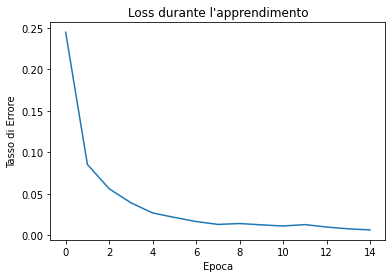
\includegraphics[width=0.50\textwidth]{CurvaApprendimentoClassica}
    \caption{Curva di Apprendimento}
\end{figure}

Dopo aver fornito alla rete anche il \textit{test pattern} per la predizione, la matrice di confusione risulta essere:

\begin{figure}[h]
    \centering
    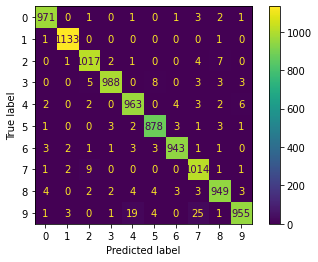
\includegraphics[width=0.50\textwidth]{MatriceConfusioneClassica}
    \caption{Matrice di Confusione}
\end{figure}

Attestando quindi una accuratezza di \(0.9811\) avendo riconosciuto 9811 valori su un totale di 10000.


\subsection{Variante Convoluzionale}

\newpage
\section{Simulazione sul Dataset Fornito}

\newpage
\section{Primo Quesito --- Numeri Difficili da Riconoscere}
\subsection{Visualizzazione di Pattern Erronei}
\subsection{Aggiunta di Rumore in Pattern Corretti}
\subsection{Visualizzazione di Pattern Erronei con Aggiunta di Rumore}

\newpage
\section{Secondo Quesito --- Variazione dell'Accuratezza su Addestramento Rumoroso}
\subsection{Accuratezza su di un Pattern di Test dopo Addestramento Rumoroso}
\subsection{Definizione di un Valore di Rumorosità Ottimale}

\newpage
\section{Terzo Quesito --- Variazione dell'Accuratezza su Pattern di Addestramento Ridotto}
\subsection{50\% del Training Set}
\subsection{25\% del Training Set}
\subsection{10\% del Training Set}


\end{document}
